% Dit werk is gelicenseerd onder de licentie Creative Commons Naamsvermelding-GelijkDelen 4.0 Internationaal. Ga naar http://creativecommons.org/licenses/by-sa/4.0/ om een kopie van de licentie te kunnen lezen.
\chapter{Stroming in leidingen}
\label{sec:Stroming in leidingen}
%%%%%%%%%%%%%%%%%%%%%%%%%%%%%%%%%%%%%%%%%%%%%%%%%%%%%%%%%%%%%%%%%%
\begin{toepassing}
	\label{buis}
Water ($\rho=1000\unit{kg/m^3}$, $\nu=1\unit{mm^2/s}$) van vloeit in een buis van \unit{40}{mm} diameter over een afstand van 500m. Het debiet is 3 liter/s.  De ruwheid van de buis is 0.046mm.
		
Bepaal de drukval over de buis voor turbulente stroming.
		
Wat zou de drukval zijn indien we er zouden in slagen om de stroming laminair te houden?
\end{toepassing}
\begin{antwoord}{\ref{buis}}
	$\Delta p = 784\unit{kPa}$, $\Delta p_{\text{laminair}} = 23\unit{kPa}$
\end{antwoord}
%%%%%%%%%%%%%%%%%%%%%%%%%%%%%%%%%%%%%%%%%%%%%%%%%%%%%%%%%%%%%%%%%%
\begin{toepassing}[*]
	\label{buisdiameter}
Een buis met ruwheid $\varepsilon = 0.0015\unit{mm}$ moet 2 liter/s water ($\rho=1000\unit{kg/m^3}$, $\nu=1\unit{mm^2/s}$) transporteren over een afstand van 400m.  Het verlies in drukhoogte mag hoogstens 30m bedragen.
		
Bepaal de minimale diameter van de buis.
\end{toepassing}
\begin{antwoord}{\ref{buisdiameter}}
	$d = 39\unit{mm}$
\end{antwoord}
%%%%%%%%%%%%%%%%%%%%%%%%%%%%%%%%%%%%%%%%%%%%%%%%%%%%%%%%%%%%%%%%%%
\begin{toepassing}
	\label{ventilatiekanaal}
Voor een ventilatiekanaal van in een vloer in een woning, waardoor een luchtdebiet van 80\unit{m^3/h} stroomt, heeft men de keuze tussen een rechthoekig kanaal met hoogte 60mm en breedte 200mm en ruwheid 0.1mm of een aantal parallelle buizen met diameter 60mm en ruwheid 0.02mm. 
		
Bepaal het aantal buizen dat nodig is om een lagere drukval te genereren. $\rho = 1.22\unit{kg/m^3}$, $\nu = 15\unit{mm^2/s}$, verwaarloos verliezen aan in- en uitstroming.
\end{toepassing}
\begin{antwoord}{\ref{ventilatiekanaal}}
	$n = 3$
\end{antwoord}
%%%%%%%%%%%%%%%%%%%%%%%%%%%%%%%%%%%%%%%%%%%%%%%%%%%%%%%%%%%%%%%%%%
\begin{toepassing}
	\label{hevel met verlies}
Een hevel wordt gebruikt om water ($\rho=1000\unit{kg/m^3}$, $\nu=1\unit{mm^2/s}$) uit een tank te halen, aan het uiteinde van de hevel heerst de atmosfeerdruk. De hoogtes zijn zoals aangegeven op onderstaande figuur, de buis heeft een constante diameter. De gebruikte buis heeft een diameter van 24mm een ruwheid van 0.1mm en een lengte van 3m, alle lokale verliezen mogen verwaarloosd worden.
		
Bepaal het debiet.

	\centering
	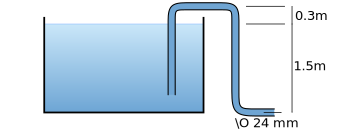
\includegraphics{/stroming_in_leidingen/hevel}
\end{toepassing}
\begin{antwoord}{\ref{hevel met verlies}}
	$\dot{V} = 67.1\unit{l/min}$
\end{antwoord}
%%%%%%%%%%%%%%%%%%%%%%%%%%%%%%%%%%%%%%%%%%%%%%%%%%%%%%%%%%%%%%%%%%%%%%%%%%%%%%%%%%%%%%
\begin{toepassing}[*]
	\label{hevel met lokale verliezen}
Bepaal voor de hevel uit Toepassing \ref{hevel met verlies} het debiet indien ook rekening gehouden wordt met de lokale verliezen veroorzaakt door de bochten.

\end{toepassing}
\begin{antwoord}{\ref{hevel met lokale verliezen}}
	$\dot{V} = 44.5\unit{l/min}$
\end{antwoord}
%%%%%%%%%%%%%%%%%%%%%%%%%%%%%%%%%%%%%%%%%%%%%%%%%%%%%%%%%%%%%%%%%%
\begin{toepassing}[*]
	\label{pompkarakteristiek}
Water ($\rho=1000\unit{kg/m^3}$, $\nu=1\unit{mm^2/s}$) wordt door een rechte leiding met binnendiameter 24mm ruwheid 0.002mm en lengte 10m van een laag reservoir gepompt naar een reservoir dat 3m hoger gelegen is. De pomp heeft een karakteristiek $H = 5 - 2*\dot{V}^2$ met $H$ uitgedrukt in meter en $\dot{V}$ in \unit{m^3/h}.

Bepaal het debiet door de leiding als alle lokale verliezen verwaarloosd mogen worden.
\end{toepassing}
\begin{antwoord}{\ref{pompkarakteristiek}}
	$\dot{V} = 2.27\unit{m^3/h}$
\end{antwoord}
%%%%%%%%%%%%%%%%%%%%%%%%%%%%%%%%%%%%%%%%%%%%%%%%%%%%%%%%%%%%%%%%%%%%%%%%%%%%%%%%%%%%
\begin{toepassing}[*]
	\label{olieafvoerdimensionering}
In een machine dient olie met een dichtheid van 830\unit{kg/m^3} en viscositeit van 240\unit{mm^2/s} afgevoerd te worden uit een carter. Door de smering van verschillende componenten stroomt er een debiet van 80l/min naar het carter. De afvoerleiding dient een pad te volgen zoals aangegeven op de tekening. Alle bochten hebben dezelfde straal als de buisdiameter. De druk in de machine en aan de olieafvoer is atmosfeerdruk.
	
Bepaal de nodige leiding diameter zodat het niveau in het carter niet hoger komt dan 500mm boven de afvoer.

	\centering
	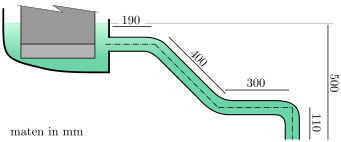
\includegraphics{fig/stroming_in_leidingen/olieafvoerdimensionering}
\end{toepassing}
\begin{antwoord}{\ref{olieafvoerdimensionering}}
	$\dot{d} = 42\unit{mm}$
\end{antwoord}
%%%%%%%%%%%%%%%%%%%%%%%%%%%%%%%%%%%%%%%%%%%%%%%%%%%%%%%%%%%%%%%%%%
\begin{toepassing}[*]
	\label{pompkarakteristiek serieschakeling}
Water ($\rho=1000\unit{kg/m^3}$, $\nu=1\unit{mm^2/s}$) wordt door leidingen zoals op de figuur aangegeven van een lager naar een hoger gelegen reservoir gepompt. Alle leidingen hebben een ruwheid van 0.5mm. De pomp heeft een karakteristiek zoals aangegeven op de figuur. De bocht heeft een gemiddelde straal van 120mm, de intrede heeft een verliescoëfficiënt $\xi = 0.1$, de uittrede heeft een verliescoëfficiënt $\xi = 0.8$.
		
Bepaal het debiet en het werkingspunt van de pomp.
		
Teken het verloop van de hoogte, snelheidshoogte, drukhoogte en het drukhoogte verlies op één figuur.

	\centering
	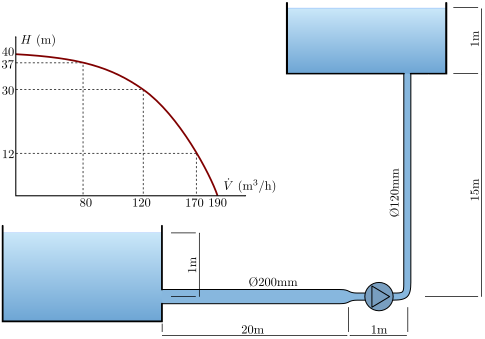
\includegraphics{fig/stroming_in_leidingen/pompopvoerhoogte}
\end{toepassing}
\begin{antwoord}{\ref{pompkarakteristiek serieschakeling}}
	$\dot{V} = 155\unit{m^3/h}$
\end{antwoord}
%%%%%%%%%%%%%%%%%%%%%%%%%%%%%%%%%%%%%%%%%%%%%%%%%%%%%%%%%%%%%%%%%%%%%%%%%%%%%%%%%%%%
\section*{Antwoorden}
	\begin{multicols}{2}
		\includecollection{antwoorden}
	\end{multicols}